% Options for packages loaded elsewhere
\PassOptionsToPackage{unicode}{hyperref}
\PassOptionsToPackage{hyphens}{url}
%
\documentclass[
]{article}
\usepackage{amsmath,amssymb}
\usepackage{lmodern}
\usepackage{iftex}
\ifPDFTeX
  \usepackage[T1]{fontenc}
  \usepackage[utf8]{inputenc}
  \usepackage{textcomp} % provide euro and other symbols
\else % if luatex or xetex
  \usepackage{unicode-math}
  \defaultfontfeatures{Scale=MatchLowercase}
  \defaultfontfeatures[\rmfamily]{Ligatures=TeX,Scale=1}
\fi
% Use upquote if available, for straight quotes in verbatim environments
\IfFileExists{upquote.sty}{\usepackage{upquote}}{}
\IfFileExists{microtype.sty}{% use microtype if available
  \usepackage[]{microtype}
  \UseMicrotypeSet[protrusion]{basicmath} % disable protrusion for tt fonts
}{}
\makeatletter
\@ifundefined{KOMAClassName}{% if non-KOMA class
  \IfFileExists{parskip.sty}{%
    \usepackage{parskip}
  }{% else
    \setlength{\parindent}{0pt}
    \setlength{\parskip}{6pt plus 2pt minus 1pt}}
}{% if KOMA class
  \KOMAoptions{parskip=half}}
\makeatother
\usepackage{xcolor}
\usepackage[margin=1in]{geometry}
\usepackage{graphicx}
\makeatletter
\def\maxwidth{\ifdim\Gin@nat@width>\linewidth\linewidth\else\Gin@nat@width\fi}
\def\maxheight{\ifdim\Gin@nat@height>\textheight\textheight\else\Gin@nat@height\fi}
\makeatother
% Scale images if necessary, so that they will not overflow the page
% margins by default, and it is still possible to overwrite the defaults
% using explicit options in \includegraphics[width, height, ...]{}
\setkeys{Gin}{width=\maxwidth,height=\maxheight,keepaspectratio}
% Set default figure placement to htbp
\makeatletter
\def\fps@figure{htbp}
\makeatother
\setlength{\emergencystretch}{3em} % prevent overfull lines
\providecommand{\tightlist}{%
  \setlength{\itemsep}{0pt}\setlength{\parskip}{0pt}}
\setcounter{secnumdepth}{5}
\newlength{\cslhangindent}
\setlength{\cslhangindent}{1.5em}
\newlength{\csllabelwidth}
\setlength{\csllabelwidth}{3em}
\newlength{\cslentryspacingunit} % times entry-spacing
\setlength{\cslentryspacingunit}{\parskip}
\newenvironment{CSLReferences}[2] % #1 hanging-ident, #2 entry spacing
 {% don't indent paragraphs
  \setlength{\parindent}{0pt}
  % turn on hanging indent if param 1 is 1
  \ifodd #1
  \let\oldpar\par
  \def\par{\hangindent=\cslhangindent\oldpar}
  \fi
  % set entry spacing
  \setlength{\parskip}{#2\cslentryspacingunit}
 }%
 {}
\usepackage{calc}
\newcommand{\CSLBlock}[1]{#1\hfill\break}
\newcommand{\CSLLeftMargin}[1]{\parbox[t]{\csllabelwidth}{#1}}
\newcommand{\CSLRightInline}[1]{\parbox[t]{\linewidth - \csllabelwidth}{#1}\break}
\newcommand{\CSLIndent}[1]{\hspace{\cslhangindent}#1}
\usepackage{multirow} 
\usepackage {enumerate} 
\usepackage{lscape}
  \newcommand{\blandscape}{\begin{landscape}} 
  \newcommand{\elandscape}{\end{landscape}}
\usepackage{float}
\let\origfigure\figure
\let\endorigfigure\endfigure
\renewenvironment{figure}[1][2] {
    \expandafter\origfigure\expandafter[H]
} {
    \endorigfigure
}
\ifLuaTeX
  \usepackage{selnolig}  % disable illegal ligatures
\fi
\IfFileExists{bookmark.sty}{\usepackage{bookmark}}{\usepackage{hyperref}}
\IfFileExists{xurl.sty}{\usepackage{xurl}}{} % add URL line breaks if available
\urlstyle{same} % disable monospaced font for URLs
\hypersetup{
  pdftitle={Decision analysis methods guide},
  pdfauthor={Eike Luedeling\^{}1; Cory Whitney\^{}1; \^{}1University of Bonn, Germany},
  hidelinks,
  pdfcreator={LaTeX via pandoc}}

\title{Decision analysis methods guide}
\usepackage{etoolbox}
\makeatletter
\providecommand{\subtitle}[1]{% add subtitle to \maketitle
  \apptocmd{\@title}{\par {\large #1 \par}}{}{}
}
\makeatother
\subtitle{Agricultural policy for nutrition}
\author{Eike Luedeling\(^1\) \and Cory
Whitney\(^1\) \and \(^1\)University of Bonn, Germany}
\date{}

\begin{document}
\maketitle

\tableofcontents
\listoffigures
\listoftables

\textbf{List of abbreviations}

\begin{itemize}
  \item Applied Information Economics (AIE)
  \item Conditional Probability Tables (CPTs)
  \item Confidence Interval (CI)
  \item Expected Monetary Value (EMV)
  \item Expected Value or perfect information (EVPI)
  \item Node Probability Table (NPT)
  \item Value of Information (VoI)
\end{itemize}

\hypertarget{summary}{%
\section{Summary}\label{summary}}

It is often very difficult to make accurate projections about how
interventions will affect the real world and to use such projections to
develop effective implementation plans, monitor progress and evaluate
project impacts. This is due to a variety of factors including lack of
data, complex impact pathways, and risks and uncertainties that are
difficult to factor into intervention planning. Scientific approaches to
produce reliable impact projections are rarely applied in agricultural
development, but Decision Analysis techniques commonly used in other
fields have the potential to improve development decisions. This manual
outlines a Decision Analysis approach that can help decision-makers
efficiently allocate resources for the most effective policy impacts.

The procedures outlined in this manual feature the construction of
causal models -- models that describe the mechanisms through which
intervention impacts will be delivered -- that are co-developed by
experts, stakeholders and analysts through facilitated participatory
processes. These models are then formalized as Bayesian Network (BN)
models, a modeling approach that has been widely applied in a range of
disciplines, including medical sciences, genetics, environmental
sciences, and legal reasoning. BNs allow for the formal representation
of causal models, such as intervention impact pathways. They can work
effectively with incomplete information, combine expert knowledge with
other sources of information, and they allow adequate consideration of
risk.

This manual illustrates the use of participatory workshops that convene
experts on the systems, stakeholders involved in ongoing or prospective
projects, and analysts. These teams can jointly develop impact pathways
for the interventions, which can be formalized into quantitative BN
models. After several rounds of feedback elicitation, and inclusion of
data from experts and other sources, stochastic simulations can be run
to determine the likely impacts of the interventions. Results can be
presented back to stakeholders for feedback.

Through the tools laid out in this manual critical uncertainties in the
models of intervention impact pathways can be identified. These
high-value variables can determine uncertainty about project outcomes.
Further measurement or dissagregation of these variables could greatly
support decision-making processes.

By demonstrating improved intervention decisions with little additional
investment and improved tools for intervention decision modeling, we
hope that this approach will be widely adopted and used to enhance the
efficacy of development activities.

\hypertarget{introduction}{%
\section{Introduction}\label{introduction}}

The development community faces increasing demand to credibly link
research and development activities with progress towards the envisioned
outcomes (Shepherd, Luedeling, \& Whitney, in preparation). Improved
planning tools for interventions that target complex systems are
urgently needed, especially in developing countries where data are
scarce and uncertainties about decision outcomes are large. However,
especially where quantitative impact predictions are requested,
stakeholders are often left guessing about development outcomes, because
they lack reliable tools to forecast impacts. Methodologies that address
these uncertainties could transform the way development is done and
greatly enhance the efficacy of its activities. Such methods could
stimulate thorough scrutiny of research priorities and direct resources
to where they lead to the greatest impacts (Luedeling \& Shepherd,
2016). For this positive effect to materialize, however, the development
community needs better approaches for planning for impact. One of the
central difficulties in planning for impact is dealing with uncertainty.
It is rarely possible to accurately predict the impacts of agriculture
for nutrition, and other types of interventions. Many of the important
factors that determine these impacts, such as adoption rates, yield
increases, the performance of a particular tree or crop in a new
environment and future weather, are highly uncertain. Additionally, many
development interventions are implemented in risky environments, where
extreme weather events, conflict, poor anticipation of cultural
preferences, political interference or other risk factors can
dramatically disrupt progress at any time (Luedeling et al., 2015).

Making impact projections in this environment, especially where precise
numbers are expected, is very difficult, and researchers and development
workers often find themselves in an ethical quagmire, torn between the
perceived need to honestly evaluate risks and the temptation to let
wishful thinking guide their estimates. The latter may lead to overly
optimistic assumptions and high impact projections that may raise the
chance of political and donor support but are essentially unrealistic.
This conflict of interest is not only a problem for project proponents
-- it also compromises the ability of stakeholders to compare impact
`promises' across proposals or reported impacts by different projects.

For research that is actually worth doing, results cannot be forecast
with certainty (otherwise the research would not be necessary). However,
what is currently lacking is a set of reliable methods to produce robust
impact projections that take into account the host of uncertainties and
risks that research and development activities are faced with. Such
methods should be based on quantitative representations of impact
pathways that capture the causal mechanisms of impact delivery. This
manual aims to provide documentation for disseminating an approach based
on Bayesian Networks (BNs) for impact pathway modeling. It seeks to
establish Bayesian Networks (BNs) as a widely used analysis tool for
development decisions related to agriculture for nutrition.

\#\#Predicting impacts of Agriculture for Nutrition activities

Many activities in agricultural research and development aim at
improving nutrition, but they are often unable to articulate clearly how
nutrition objectives will be achieved and to what degree. Agricultural
systems in developing countries are complex, and few agricultural
interventions can be expected to impact such systems in a linear way.
Thus there is a need for new approaches for analyzing the impacts of
agricultural interventions on food and nutrition systems.

The success of an intervention will always depend on a number of factors
that interact in ways that would be difficult or impossible to predict
with precision. Some examples of these difficult-to-measure factors are
the so-called `intangible' factors, such as people's perceptions of
healthy food and their food preferences. The nutritional status of a
country's population is determined by many such factors, including, of
course, the nutritional value of the food people eat, but also a complex
interplay between the food environment, household economics, health,
education, and agricultural value chains (Waage, Hawkes, \& Turner,
2012). Thus, many pathways may have the potential to improve national
nutrition, e.g.~through higher nutrient contents in crops (DellaPenna,
1999; Nestel, Bouis, Meenakshi, \& Pfeiffer, 2006), greater nutritional
diversity (Hoddinott \& Yohannes, 2002) or improved awareness about
childhood nutrition (Ruel, Alderman, \& Maternal, 2013). For any given
context, however, it is difficult to decide \emph{a priori}, which
pathway will be most effective. Some pathways may not produce positive
outcomes at all, if, for instance, the value chain degrades the
nutritional value of the food, or if certain foods never reach
vulnerable groups (e.g.~children or lactating women).

Credible impact pathways regarding agriculture for nutrition should
reflect their complexity. However, there is currently a severe shortage
of practical methods that allow credible analysis of these complex
systems. Most conventional scientific approaches are unable to deal with
this complexity. Opportunities for controlled trials are very limited,
especially at low cost, and simple statistical tools (regressions,
correlations) do not provide much information about the way that drivers
of agricultural systems are related to nutritional (and other) outcomes.

Use and analysis of impact pathways have helped to show how
interventions function, where they are lacking and what can be done to
improve them. Leroy, Ruel, \& Verhofstadt (2009), for example, used
impact pathway models to review the effect of cash transfer programs on
child nutrition outcomes. Olney, Talukder, Iannotti, Ruel, \& Quinn
(2009), used impact pathway models to evaluate the maternal and child
health and nutrition effects of a homestead food production program in
Cambodia and found that household-level benefits from the program did
not translate into significant improvements in maternal and child health
and nutrition. Both studies found a major gap in implementer and
stakeholder knowledge about how the programs improve nutrition and
identified this as a major obstacle to the interventions.

This manual provides a step by step guide to help synthesize expert
knowledge and other sources of information into BN models that provide
credible probabilistic projections of the impact of decisions. The
methods described can be applied to multiple nutrition outcomes. The
resulting models, as well as the participatory process from which they
emerge, can be used to define useful metrics for monitoring progress
towards nutrition outcomes. To achieve this, this manual demonstrates a
Bayesian approach, which seeks to express the current state of
uncertainty on everything that matters to a decision, can help to focus
the measurement effort on areas that can narrow uncertainty to reduce
ambiguity in the decision. Analysts can then update BNs based on the new
information. Whether a factor is seemingly easy or difficult to measure
or has existing data available has no bearing on its inclusion. Omitting
an important factor is essentially prescribing it as valueless. This is
then complemented with innovative group work techniques for eliciting
expert knowledge to construct a logical framework to describe system
interactions and outcomes (i.e.~an impact pathway). Expert knowledge is
thereby used to generate BN model structures (Bolger \& Rowe, 2015;
Kuhnert, Martin, \& Griffiths, 2010; Papakosta, Xanthopoulos, \& Straub,
2017) and these are then integrated into model calculations (cf. Yet et
al., 2016).

\#\#Decision Analysis

Decision Analysis provides a framework for development research. Its
objective is to facilitate better decisions by gaining insights into
what actions could most increase multiple benefits given stakeholder
preferences, while minimizing costs and risks. Abbas \& Howard (2015)
illustrate how the foundations of Decision Analysis provide the norms
for decision making. The basic Decision Analysis approach seeks to
increase benefits and decrease risks on a continuous basis through the
intervention planning and implementation process. The insights gained
through the Decision Analysis approach include better understanding of
the magnitude of the trade-offs among different development objectives
relative to the preferences of different stakeholder groups. The
ultimate aim is to lead to clarity of action for decision makers

The basic steps in the Decision Analysis process, see
\autoref{Fig_Diagram_Shepherd}, address the questions of both why and
how decisions are formulated and factors are measured. Hubbard\_2014
outlines some of these approaches as part of his Applied Information
Economics (AIE), which he calls the `Universal Modeling Approach', since
AIE has the basic premise that if something has an affect, it must be
observable, and if it is observable it must be measurable. Decision
Analysis and AIE are a collection of decision theory and risk analysis
tools which use:

\begin{itemize}
  \item calibrated probability assessment (discussed in more detail in \autoref{calibration-training}) 
  \item value of additional information calculations applied to uncertain variables in a decision model, the results of which will reveal where to focus efforts to reduce uncertainty (e.g. by model refinement or by making further measurements).
  \item empirical methods applied according to the information value of the measurement. 
\end{itemize}

\autoref{Fig_Diagram_Shepherd} shows a technical diagram of the Decision
Analysis process adapted from Shepherd et al. (in preparation). The
process outlined is followed in cooperation with key stakeholders and
experts to improve the design of policy and interventions and monitor
their impacts. The loop in the top half of the diagram describes the
process that evaluates different alternatives in relation to the
decision goals, whereas the lower loop uses value of information
analysis to determine what should be measured to clarify the decision.
There are iterative feedback loops throughout the process.

\begin{figure}
\centering
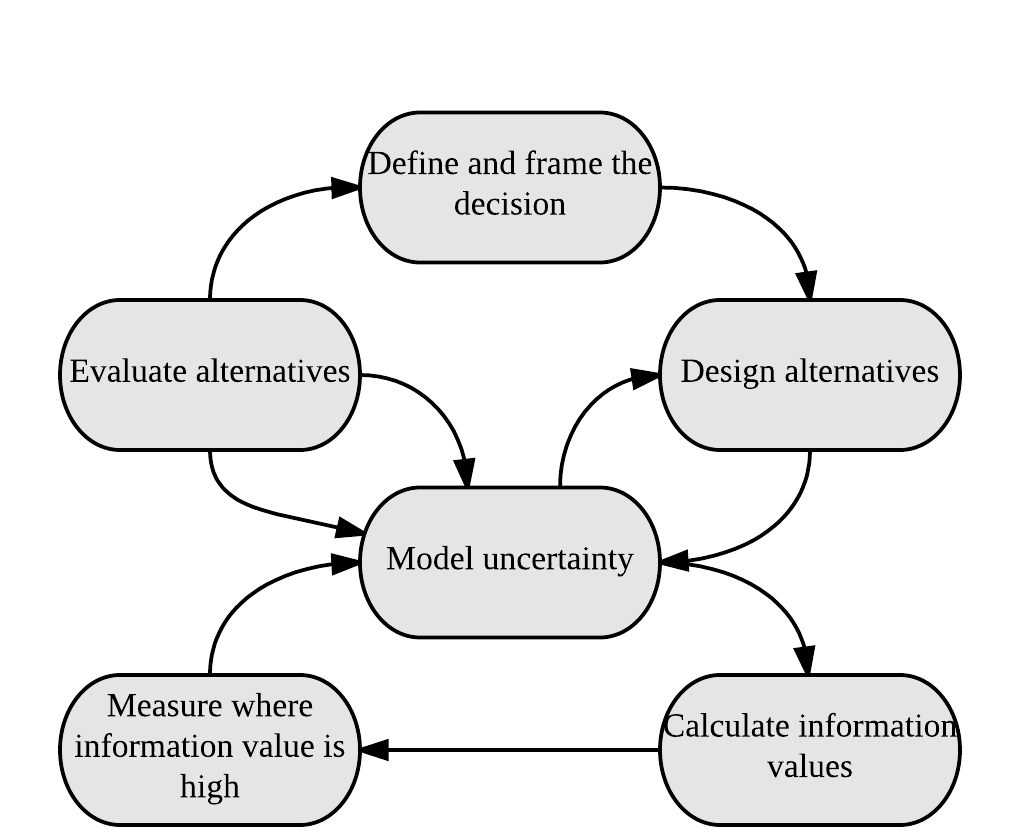
\includegraphics{Fig_Diagram_Shepherd.png}
\caption{Summary of the decision modeling proces; the sequence of
activities in the decision modeling approach (adapted from Shepherd et
al.~in preperation).\label{Fig_Diagram_Shepherd}}
\end{figure}

The merits of the application of the Decision Analysis tools for
development decisions have been further described in detail. Luedeling
\& Shepherd (2016) point out that Decision Analysis solves the problem
of data gaps, which has often prevented research from comprehensively
and holistically forecasting decision impacts. It also allows explicit
consideration of risks and variability.

Decision Analysis tools allow for decision making that draws on all
appropriate sources of evidence rather than rule out intangible and hard
to measure aspects of a decision. Luedeling \& Shepherd (2016) point out
that, in Decision Analysis, a model should include all the factors and
all the important decision impacts that experts consider relevant,
regardless of data availability. Shepherd et al. (2015) points out that
Decision Analysis tools are particularly useful in development contexts,
where data are often sparse. One very useful aspect of the approach is
that expert knowledge can be used to fill in the knowledge gaps and
avoid missing important factors when deciding about development
interventions.

\#Steps in the Decision Analysis process

\#\#Decision framing

Decision framing is the first part of the decision analysis process, it
determines the boundaries of a decision and is the most important aspect
of making a good decision. Decision framing starts by identifying both a
decision to be modeled and the relevant experts. This is not as simple
as it sounds and should be undertaken carefully and with a lot of
forethought. Consideration of the criteria which define a decision can
help to help add structure to this important step in the process:

\begin{itemize}
  \item it is a choice between two or more alternatives that involves an irrevocable allocation of resources, 
  \item it involves uncertainty (as we pointed out earlier the analysis would not be necessary if results could be forecast with certainty).
  \item it involves a decision maker or decision making body (who will allocate resources or act).
\end{itemize}

As Shepherd et al. (in preparation) points out, in order to to achieve
clarity in decision making each of the above elements, and the
preferences of the decision maker, need to be carefully defined.

Once the decision has been identified, the decision analysts then
identify and convene relevant decision-makers, stakeholders, and any
additional experts. We find that around 20 experts makes for a
manageable workshop, more can be cumbersome, especially when dealing
with model building in plenary.

It is important to have a number of different types of knowledge holders
involved in the development of the impact model. Therefore, expert
selection should seek to gather experts with knowledge on as many
aspects of the decision as possible. As Fenton \& Neil (2012) points
out, expert knowledge is often vital in identifying critical, underlying
causal factors that affect risks and opportunities that would otherwise
have been missed based on available data or statistical models. The
experts selected for modeling agriculture for nutrition decisions should
represent a mix of knowledge holders such as academic institutions
(e.g.~nutritionists and agronomists), government institutions, local
villages and development organizations (see Luedeling, 2017).

\#\#Generating a graphical model

The next step in the Decision Analysis process is to jointly develop a
decision model (\autoref{Fig_Diagram_Shepherd}). In the workshop setting
it is important for the analyst to gather all the variables that the
expert group agrees are logically important to describe the impact
pathway of the decision and include them in the model. This should be
done regardless of the ease of measurement of the individual variables.

Before engaging in this process the overall context for the model (the
decision that was identified) should be defined explicitly and agreed
upon in plenary discussions with the identified experts. Once this has
been done, building the graphical model can begin. In our approach we
start from the decision framing step through to the model development by
asking experts to work together and peer review each others work.

Bolger \& Rowe (2015) and Bolger \& Wright (2017) point out the various
challenges in handling expert knowledge, which include both poor
judgment regarding probability and high levels of variation among
experts. These problems occur because experts are not trained to
formulate reliable representations of uncertainty, many lack experience
with probability and few learn to express their uncertainty as
probability distributions. Here we outline several important steps that
should be taken to aid in the process of collaboratively building model
structures and making variable estimates. These will help to ensure
accuracy in the process.

\#\#\#Colaborative approaches

Tools are available to help overcome these problems. According to Bolger
\& Rowe (2015) it is possible to create better conditions for gathering
expert knowledge. These include offering experts experiences in making
estimates for well-defined targets, offering tools on which to base
their estimates, and offering regular and usable feedback about the
accuracy of their estimates. Bolger \& Wright (2017) experts can be a
source of quality data about the future. Ensuring the quality of this
data starts by selecting the best experts, training experts in the
normative aspects of anticipation and combining judgments from several
experts.

Here we illustrate some useful approaches for combining experts
probability distributions, using the accumulated information from
multiple experts. In this approach a workshop is held and graphical
models are developed by individual experts and then peer reviewed by
other experts. These approaches allow analysts to obtain as much
information as possible and gather data that represent a summary of
expert opinion. More examples of these tools in practice are shown by
Clemen \& Winkler (1999) and Bolger \& Wright (2017).

\autoref{Fig_Elicit_Proc} has been adapted from Whitney et al. (in
preparation), it illustrates a process that can be used for eliciting
graphical representations of decisions from expert groups to be used in
developing a BN. This approach is generally outlined in the work of
Iqbal \& MacLean (2010), who consulted experts in repeated group
meetings to build a BN for defoliation prediction by sawfly infestations
in Newfoundland. Each expert was asked to create a BN model and this was
then peer reviewed by other experts. In our approach the process begins
with breaking the decision down into several important questions in
plenary discussions. Random interchanging working groups of experts are
then led through three stages of collaborative thinking for each
question that is brought up, these are:

\begin{enumerate}
  \item Consider the question alone. Experts are given a short time (usually a minute or two) for quiet reflection and writing on the question
  \item Share with immediate neighbor. Experts are given some time (usually a few minutes) to compare notes and ideas on the question with another participant in the working group.
  \item Share with working group and design. Working groups are given as much time as necessary to discuss and design a model of their collective understanding of the functional pathways related to the question.
\end{enumerate}

The steps defined above and shown in \autoref{Fig_Elicit_Proc} are
designed to help experts interact, brainstorm and help reach common
understanding about impact pathways. Through this approach, experts can
explore details of the expected impacts, disaggregate the impact pathway
into the intermediate steps and identify all the influencing factors
that they consider important to the decision (i.e.~draw a model of nodes
and edges; cf.~\autoref{Fig_UG_BN}).

\begin{figure}
\centering
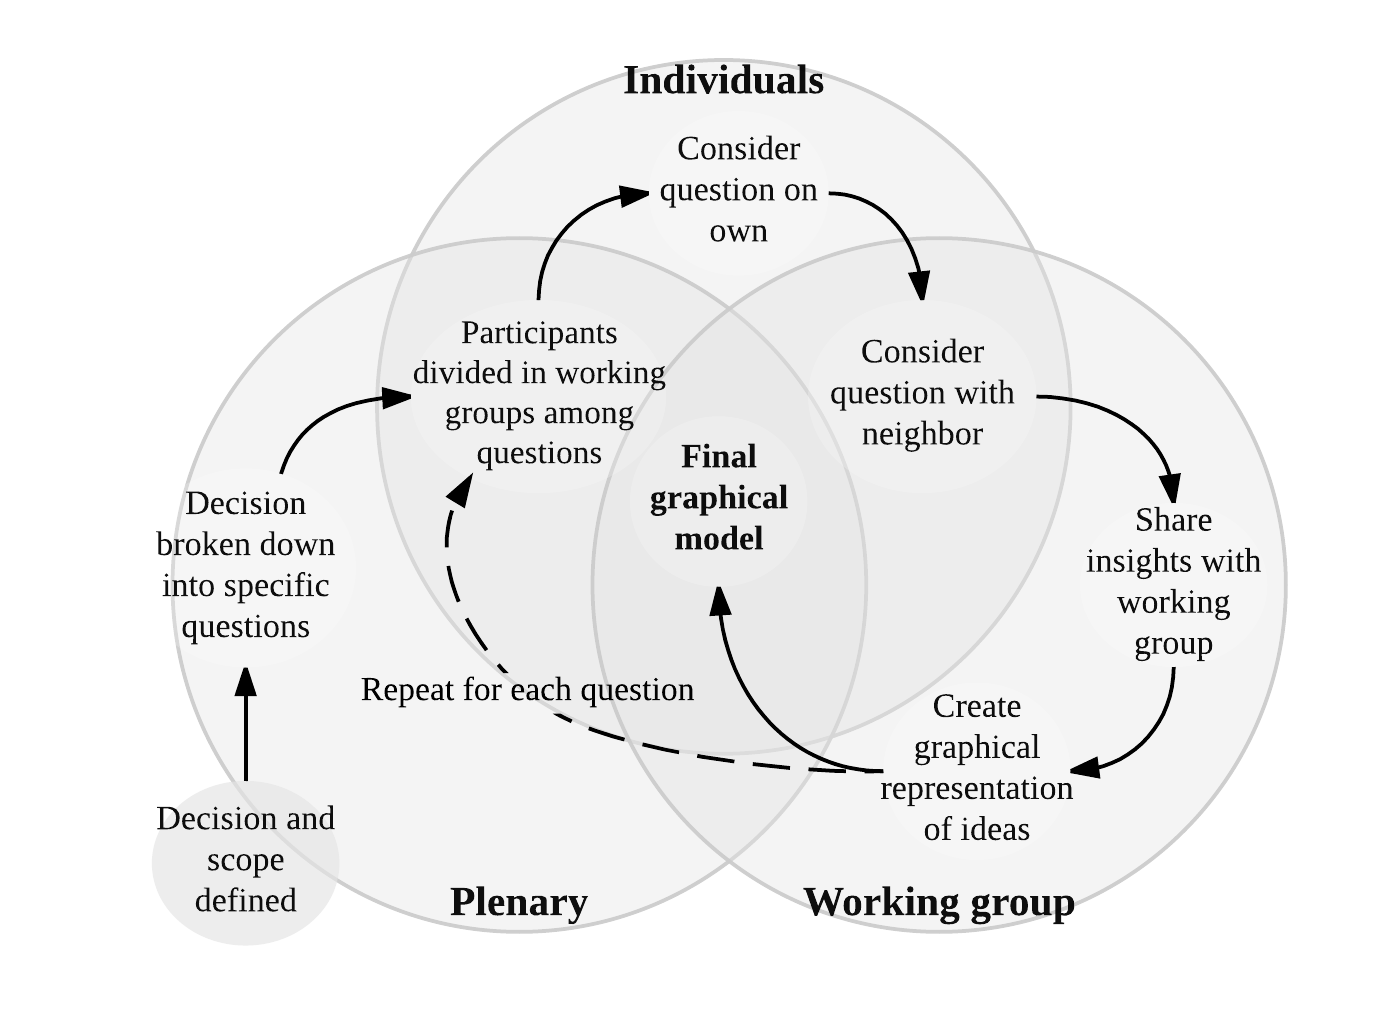
\includegraphics{Fig_Elicit_Proc.png}
\caption{Process used for eliciting graphical representations of
decisions from expert groups to be used in developing a
BN\label{Fig_Elicit_Proc}}
\end{figure}

The steps shown in \autoref{Fig_Elicit_Proc} are repeated until all
experts have worked on each question and are satisfied that all specific
relationships have been identified. This iterative process of building a
model in the workshop is illustrated conceptually in
\autoref{Fig_Elicit_Proc}. Participants should be encouraged to discuss
any factors they deem important for the decision, in particular the
various costs, benefits, and risks associated with interventions, as
well as the objectives and concerns of decision-makers and stakeholders.
The model should have the broad aim to describe the effects of
agricultural decisions on specific nutrition outputs such as hunger
(a.k.a. global energy and macronutrient deficiency).

Following this approach, it is important that the analysts have an
overview of the process with the objective of building a final working
BN model in mind. Analysts should work to guide the experts so that they
think about how model parameters interact in a logical way. For example
the work of Whitney et al. (in preparation) illustrates the use of the
EKE approach to build an impact model which aims to deliver the
probabilities for different states of malnutrition under a policy
decision and to relate this directly to a monetary value for calculating
variables of importance (see \autoref{multivariate-analysis})

Resulting models can then be brought before the whole group of experts
for plenary discussion and re-drawn, aiming for common understanding
about the relationships in each model. The end result should be one
model per question with the contributions of all experts. These can then
be combined into one large impact pathway model. Corrections and further
feedback can be gathered for model verification as a final stage of
model development.

\#\#Calibration training

The next step of the modeling procedure follows procedures, outlined by
Hubbard (2014), known as `calibration training'. Experts are trained,
using well-established `calibration' procedures to estimate their state
of uncertainty and thereby increase their capacity to provide accurate
estimates by reducing errors of judgment. Through the process, experts
learn to improve their ability to estimate their own state of
uncertainty and thereby reduce errors of judgment, e.g.~under-confidence
or overconfidence (i.e.~give correct estimates 90\% of the time when
they have 90\% confidence, Hubbard, 2014). As both Hubbard (2014) and
O'Hagan et al. (2006) show, through this training the experts learn to
minimize potential biases in probability estimation.

Calibration training consists of several exercises aiming to reveal to
the participants their personal biases (overconfidence or
underconfidence) by assessing their performance on a set of trivia
questions. Through these exercises experts are trained to assess their
subjective uncertainty and express it as a Confidence Interval (CI).
This interval has a predefined chance (e.g.~90\%) of containing the
right value. Perfectly calibrated people should get around 90\% of
answers correct, and any deviation (outside a narrow band of stochastic
variation) from this optimal figure indicates estimation bias. Experts
are calibrated through repetition and feedback on the exercises. The
training is divided into several stages:

\begin{enumerate}
  \item The concepts of calibration are presented to the participants, along with the empirical evidence that assessing uncertainty is not a skill that arises automatically from experience but a general skill that can be gained through training in quantification techniques.
\item Participants benchmark their “natural” skills in quantifying their own uncertainty. To this end, they take a short quiz aimed to help them determine their initial level of overconfidence.
\item Methods of self-calibration proposed by Hubbard (2014), are provided such as: 
\begin{itemize}
  \item The “equivalent bet test”: Participants are invited to imagine a spinning dial on a circle that is 10% red and 90% green. They are asked to imagine that if the real answer falls within the range they selected, they win 100 dollars, or they can choose to spin the dial and if the arrow lands on green are they win 100 dollars. If they prefer the dial over the wheel they do not have 90% confidence in their answer (overconfident) and if they choose their answer instead of the wheel, their confidence level is higher than 90% (underconfident). 
  \item The test of “considering two pros and two cons”: Participants are invited to imagine that the limits that they provided for their estimate range are wrong. They then consider different possible explanations for thy these are wrong and, if any insights arise, they adjust accordingly.  
  \item The “absurdity test”: Participants are invited to create distributions that they are sure are wildly broader than the actual 90% confidence range. They then slowly reduce their ranges down to a more reasonable distribution while considering the logic behind the reduction.
  \end{itemize}
\item Participants work on two types of exercises: (1) 90% CI questions and (2) binary questions. In the 90% CI questions, they are asked to provide a range (a lower bound and an upper bound) for which there is a 90% chance that it includes the right answer. In the binary questions, they answer whether each of a series of statements is true or false and then give the probability they think their answer is the right one. This is an iterative process: they give their answers, compare with the true values and test again.
\end{enumerate}

The examples given by Hubbard (2014) and Luedeling et al. (2015) show
that through the use of these procedures, experts learn to give
estimates that are neither too vague (under-confidence) or too specific
(overconfidence). The procedures seek to help participants become
accurate estimators. Accuracy, in this context, does not mean precision
but rather refers to the ability to produce an accurate range of
probable estimates of different possible states of the variables of
interest. Therefore, the procedures outlined in this appraoch seek to
provide experts with the skills necessary to represent uncertainty
explicitly as probabilities of different possible states of the world.

Estimations of the nodes states within the BN can begin once the experts
have been through the training and the analysts are satisfied that the
experts are adequately calibrated. More examples of these calibration
procedures and instructions on their application is provided in detail
by Hubbard (2014).

\#\#Model quantification

For final model quantification the analyst converts the conceptual model
into a mathematical model, translating stakeholder inputs into equations
as accurately as possible. Following Luedeling et al. (2015), all
estimates can then be consolidated into one single distribution for each
model parameter.

Once completed and verified with the literature and other sources, the
BN can be shared with experts again for verifying its logical
consistency and receiving final feedback.

\#\#Value of Information analysis

As we said in \autoref{generating-a-graphical-model} it is important for
the analyst to gather all the variables that the expert group agrees are
logically important to describe the impact pathway of the decision and
include them in the model. This should happen for several reasons, the
most important of which is that the final development outcomes are
generally strongly dependent on variables with high uncertainty. These
intangible and uncertain variables often include important factors such
as behavioral, institutional and policy factors, and are likely to be
brought up by the experts as part of their discussions of impact
pathways. Part of the value of the Decision Analysis approach is that it
directs attention and performance monitoring to such factors, identified
by their high information value.

When a model has been programmed in the approproate software and no
clearly preferable option emerges from teh model results, Value of
Information (VoI) analysis is a tool that can be used to reveal what
further information is needed to narrow uncertainty and clarify a
decision. It is expressed as the amount that a rational decision-maker
would be willing to pay for that knowledge before making a decision. VoI
is a central concept of Decision Analysis, it is used to guide decisions
on the level of complexity to be considered in a decision model and the
need for further measurement to clarify decision alternatives. VoI can
be estimated by analyzing the uncertainties in all the variables that
have a bearing on a decision. According to Abbas \& Howard (2015) VoI
could also be called the value of clairvoyance.

VoI analysis can be used to determine whether additional information on
certain input variables in the BN model could increase confidence about
the emerging decision recommendation. The examples of Hubbard (2014)
show that when value of information analysis is used to prioritize
measurements, it is often found that only a few variables may be
relevant, and data collection should focus on those that narrow choices
the most. Other examples, such as those of Constantinou, Yet, Fenton,
Neil, \& Marsh (2016) and Whitney et al. (2017), illustrate how the
results of VoI analysis can be used for prioritizing knowledge gaps that
should most urgently be narrowed in order to improve certainty about a
decision. Constantinou et al. (2016) also show that VoI can help
decision makers learn if a decision outcome is dependent on, or
independent of any risk factors, thereby helping to focus any necessary
follow-up research resources. More follow-up measurements and
disaggregation of any identified variables can help inform the design
and prioritization of future research and provide guidance about the
best pathways for implementing the current decision.

\#\#\#Expected Value of Perfect Information

The Expected Value of Perfect Information (EVPI) is one useful VoI tool.
It is the difference between the expected value of a decision made with
perfect information and the expected value of the decision with current
imperfect information (Hubbard, 2014). The many examples presented by
Hubbard (2014) and those of Felli \& Hazen (2003) show how EVPI can help
decision makers to consider both the probability of changes due to a
decision, and the resulting difference in payoff. Constantinou et al.
(2016) show how EVPI can be calculated for BN models to identify a
selected subset of important model variables. To achieve this, utility
nodes are used to assign monetary value to model outputs (example shown
in \autoref{Table_EVPI_calc}).

The Expected Monetary Value (EMV) is a key part of the EVPI calculation.
It is the weighted average of the payoffs for a decision alternative,
where weights are the probabilities of the different states of nature
(\autoref{Table_EVPI_calc}). EVPI is the maximum amount that one should
be willing to pay for additional information about the decision.
\(EVPI = EV with PI – max(EMV)\), i.e.~it is the expected value for the
decision (payoff) if perfect information is available about the states
of nature, minus the expected value for the decision if perfect
information is not available.

A simple hypothetical example of a Value of Information (VoI)
calculation, based on the Ugandan nutrition example, is given in
\autoref{Table_EVPI_calc}. This model is shown in \autoref{Fig_UG_BN}
and available on the Harvard DataVerse (Luedeling, 2017). The table is
populated with estimated values for different states of the
\emph{Diversity of household diets} based on the implementation of
Vision 2040.

\autoref{Table_EVPI_calc} shows the calculation of EVPI in a BN. The
main part of the table is populated with a `utility value' for diverse
diets under each of the `states of nature', e.g.~the upper right value
of -4 represents the utility value of low household dietary diversity in
the scenario where the decision to implement Vision 2040 is not taken.
The likelihood of each of the states of \emph{Diversity of household
diets} is shown in the row labeled with \emph{Probability}.

In \autoref{Table_EVPI_calc} EMV is calculated for each state of the
Vision 2040 decision by adding the utility values after multiplying them
by the probability for each state of \emph{Diversity of household
diets}. The maximum EMV is the highest of these two (27.7). Expected
value with perfect information (EV with PI) is calculated for each
column by selecting the highest value for each state of \emph{Diversity
of household diets} (29.7). EVPI is calculated using the resulting
values \(EVPI = EV with PI – max(EMV)\).

\begin{table}[]
\centering
\caption{Example table for calculation of the expected value of perfect information (EVPI) for a Bayesian Network model of utility values for value of diverse diets.}
\label{Table_EVPI_calc}
\begin{tabular}{lllll}
\hline
 & \multicolumn{3}{l}{Diversity of household diets} & \multicolumn{1}{c}{\multirow{2}{*}{Expected Monetary Value (EMV)}} \\ \cline{1-4}
States & Low & Medium & High & \multicolumn{1}{c}{} \\ \cline{5-5} 
Vision 2040 implemented & \textbf{-4} & \textbf{42} & 60 & EMV = 0.35(-4)+0.55(42)+0.1(60)=\textbf{27.7} \\
Vision 2040 not implemented & -11 & 31 & \textbf{80} & EMV = 0.35(-11)+0.55(31)+0.1(80)=\textbf{21.2} \\
Probability & 0.35 & 0.55 & 0.1 & Maximum EMV = \textbf{27.7} \\
EV with PI & \multicolumn{3}{c}{0.35(-4)+0.55(42)+0.1(80)=\textbf{29.7}} &  \\
EVPI & \multicolumn{3}{c}{29.7-27.7=\textbf{2}} &  \\ \hline
\end{tabular}
\end{table}

Variables that have large uncertainty and a large potential impact on
outcomes will have high information values. Information values also
point decision makers to places where they could adjust the intervention
design to reduce risks and improve outcomes, and also where to increase
model complexity. With the new information, the model can be run again
and the process is repeated until decision makers feel confident that
they can make a well-informed decision \autoref{Fig_Diagram_Shepherd}.

Value of information analysis provides an efficient, iterative approach
to information collection, as measurements are only made as far as
needed and lowest cost options are tried first. As a first step \ldots{}
decomposing model variables into sub-variables that are easier to
estimate in an attempt to narrow uncertainty. If there is still residual
information value, then the analysts may try further literature review
or consulting with more experts to further narrow the uncertainty.

In this approach analysts only need to design physical measurements or
surveys if the other steps are insufficient. Even in the case that more
data needs to be gathered, small sample sizes may be sufficient to
reduce uncertainty and reveal a clear decision. Value of information
analysis also tells decision makers how much they should consider
spending on these measurements. From applying probabilistic decision
modeling on over 80 diverse problems, Hubbard (2014) observed that only
a few variables typically had high information value in any given
decision, and interestingly they were rarely variables receiving current
measurement effort.

\#The decisionSupport package

The decisionSupport package (Luedeling \& Goehring, 2017) in the R
programming language (Team, 2017) performs several useful functions for
the development of BNs. One particularly useful tool is the likelihood
method for estimating CPTs. The the likelihood method works by defining
the likelihood that states of several qualitative variables lead to
states of another qualitative one.

\#\#The decisionSupport package

The reader may also find it useful to explore the integration of these
BN approaches within a Monte Carlo analysis. Monte Carlo is another
commonly used Decision Analysis tool. It can be combned with BN. We will
not give an exhaustive explaiantion of the implementation of these tool
shere but have descibed them in deail in an umber of publications and
through the vignette in the (Luedeling \& Goehring, 2017) in the R
programming language (Team, 2017). good implementation of that
\textbf{RPUBS CITATION}

\#Conclusions

In this manual we have attempted to outline some tools for the
adaptation and application of Bayesian Networks to agriculture for
nutrition development contexts. Decision Analysis is an important
paradigm for development research. The approach of using BN models
promises to be an effective strategy for dealing with complex systems,
multiple impact pathways, uncertain and incomplete information, and
other current constraints to meaningful quantitative impact projections.

The many factors that determine the nutritional impact of agricultural
interventions are interconnected in various ways, and there are often
clear causal connections between them. Most traditional research
approaches, such as regression analysis, controlled trials etc. fare
poorly in complex and multi-factorial situations, and results from
modeling exercises that adopt deterministic perspectives on complex
systems are often not credible because they rely on a host of
simplifying assumptions. However, rational prioritization among
`agriculture for nutrition' actions requires an evaluation approach that
can accommodate the complex relationships and thereby credibly translate
agricultural activities into nutritional outcomes.

We see the potential for great benefits to arise from an approach such
as BNs within the Decision Analysis paradigm. These approaches can
integrate existing data with expert opinion and other sources of
information. This can be a considerable improvement in development
research, especially for considering causal relationships in potential
intervention impacts. We hope that this manual will contribute to the
wider application of these tools to agriculture for nutrition decisions.

More information and resources are available through the referenced
materials, in the decisionSupport package for R (Luedeling \& Goehring,
2017) and the AgenaRisk software (Fenton \& Neil, 2016), as well as on
the Harvard DataVerse (Luedeling, 2017).

\#References

\hypertarget{refs}{}
\begin{CSLReferences}{1}{0}
\leavevmode\vadjust pre{\hypertarget{ref-Abbas_2015}{}}%
Abbas, A. E., \& Howard, R. A. 2015. \textbf{\emph{Foundations of
decision analysis}}: 832. NY, NY: Prentice Hall.

\leavevmode\vadjust pre{\hypertarget{ref-Bolger_2015}{}}%
Bolger, F., \& Rowe, G. 2015. The aggregation of expert judgment: Do
good things come to those who weight. \textbf{\emph{Risk Analysis}},
35(1): 5--11.

\leavevmode\vadjust pre{\hypertarget{ref-Bolger_2017}{}}%
Bolger, F., \& Wright, G. 2017. Use of expert knowledge to anticipate
the future: Issues, analysis and directions. \textbf{\emph{International
Journal of Forecasting}}, 33(1): 230--243.

\leavevmode\vadjust pre{\hypertarget{ref-Clemen_1999}{}}%
Clemen, R. T., \& Winkler, R. L. 1999. Combining probability
distributions from experts in risk analysis. \textbf{\emph{Risk
Analysis}}, 19(2): 187--203.

\leavevmode\vadjust pre{\hypertarget{ref-Constan_2016}{}}%
Constantinou, A., Yet, B., Fenton, N., Neil, M., \& Marsh, W. 2016.
Value of information analysis for interventional and counterfactual
bayesian networks in forensic medical sciences. \textbf{\emph{Artificial
Intelligence in Medicine}}, 66: 41--52.

\leavevmode\vadjust pre{\hypertarget{ref-Della_1999}{}}%
DellaPenna, D. 1999. Nutritional genomics: Manipulating plant
micronutrients to improve human health. \textbf{\emph{Science}},
285(5426): 375--379.

\leavevmode\vadjust pre{\hypertarget{ref-Felli_2003}{}}%
Felli, J. C., \& Hazen, G. B. 2003. Sensitivity analysis and the
expected value of perfect information. \textbf{\emph{Medical Decision
Making}}, 23(1): 97.

\leavevmode\vadjust pre{\hypertarget{ref-Fenton_2012}{}}%
Fenton, N., \& Neil, M. 2012. \textbf{\emph{Risk assessment and decision
analysis with bayesian networks}}: 503. Boca Raton, Florida: CRC Press.

\leavevmode\vadjust pre{\hypertarget{ref-Agena_V7_2016}{}}%
Fenton, N., \& Neil, M. 2016. AgenaRisk professional version 7.0.
\textbf{\emph{Revision 3451 VOI}}.

\leavevmode\vadjust pre{\hypertarget{ref-Hoddinott_2002}{}}%
Hoddinott, J., \& Yohannes, Y. 2002. \textbf{\emph{Dietary diversity as
a food security indicator}}, vol. Discussion Paper 136: 1--2.
Washington, DC: International Food Policy Research Institute (IFPRI).

\leavevmode\vadjust pre{\hypertarget{ref-Hubbard_2014}{}}%
Hubbard, D. W. 2014. \textbf{\emph{How to measure anything: Finding the
value of intangibles in business}}, vol. Second Edition: 301. Hoboken,
New Jersey: John Wiley \& Sons.

\leavevmode\vadjust pre{\hypertarget{ref-Iqbal_2010}{}}%
Iqbal, J., \& MacLean, D. A. 2010. Prediction of balsam fir sawfly
defoliation using a bayesian network model. \textbf{\emph{Can. J. For.
Res.}}, 40(12): 2322--2332.

\leavevmode\vadjust pre{\hypertarget{ref-Kuhnert_2010}{}}%
Kuhnert, P., Martin, T., \& Griffiths, S. 2010. A guide to eliciting and
using expert knowledge in bayesian ecological models.
\textbf{\emph{Ecology Letters}}, 13(7): 900--914.

\leavevmode\vadjust pre{\hypertarget{ref-Leroy_2009}{}}%
Leroy, J. L., Ruel, M., \& Verhofstadt, E. 2009. The impact of
conditional cash transfer programmes on child nutrition: A review of
evidence using a programme theory framework. \textbf{\emph{Journal of
Development Effectiveness}}, 1(2): 103--129.

\leavevmode\vadjust pre{\hypertarget{ref-Luedeling_Dataverse_2016}{}}%
Luedeling, E. 2017. Probabilistic causal models for nutrition outcomes
of agricultural actions - uganda model. \textbf{\emph{Harvard Dataverse,
World Agroforestry Centre - ICRAF Dataverse, ICRAF Decision Analysis
Dataverse}}.

\leavevmode\vadjust pre{\hypertarget{ref-decisionSupport_2017}{}}%
Luedeling, E., \& Goehring, L. 2017. \textbf{\emph{decisionSupport --
quantitative support of decision making under uncertainty. Contributed
package to the r programming language. Version 1.103.2}}.

\leavevmode\vadjust pre{\hypertarget{ref-Luedeling_Wajir_2015}{}}%
Luedeling, E., Oord, A. L., Kiteme, B., Ogalleh, S., Malesu, M., et al.
2015. Fresh groundwater for wajir - ex-ante assessment of uncertain
benefits for multiple stakeholders in a water supply project in northern
kenya. \textbf{\emph{Frontiers in Environmental Science}}, 3, article
16: 1--18.

\leavevmode\vadjust pre{\hypertarget{ref-Luedeling_Solutions_2016}{}}%
Luedeling, E., \& Shepherd, K. 2016. Decision-focused agricultural
research. \textbf{\emph{Solutions}}, 7(5): 46--54.

\leavevmode\vadjust pre{\hypertarget{ref-Nestel_2006}{}}%
Nestel, P., Bouis, H. E., Meenakshi, J., \& Pfeiffer, W. 2006.
Biofortification of staple food crops. \textbf{\emph{The Journal of
Nutrition}}, 136(4): 1064--1067.

\leavevmode\vadjust pre{\hypertarget{ref-Ohagan_2006}{}}%
O'Hagan, A., Buck, C. E., Daneshkhah, A., Eiser, J. R., Garthwaite, P.
H., et al. 2006. \textbf{\emph{Uncertain judgements: Eliciting experts'
probabilities}}. West Sussex: John Wiley \& Sons.

\leavevmode\vadjust pre{\hypertarget{ref-Olney_2009}{}}%
Olney, D. K., Talukder, A., Iannotti, L. L., Ruel, M. T., \& Quinn, V.
2009. Assessing impact and impact pathways of a homestead food
production program on household and child nutrition in cambodia.
\textbf{\emph{Food and Nutrition Bulletin}}, 30(4): 355--369.

\leavevmode\vadjust pre{\hypertarget{ref-Papakosta_2017}{}}%
Papakosta, P., Xanthopoulos, G., \& Straub, D. 2017. Probabilistic
prediction of wildfire economic losses to housing in cyprus using
bayesian network analysis. \textbf{\emph{International Journal of
Wildland Fire}}, 26(1): 10--23.

\leavevmode\vadjust pre{\hypertarget{ref-Ruel_2013}{}}%
Ruel, M., Alderman, H., \& Maternal, C. N. S. G. 2013.
Nutrition-sensitive interventions and programmes: How can they help to
accelerate progress in improving maternal and child nutrition.
\textbf{\emph{Lancet}}, 382(9891): 536--551.

\leavevmode\vadjust pre{\hypertarget{ref-Shepherd_2015}{}}%
Shepherd, K., Hubbard, D., Fenton, N., Claxton, K., Luedeling, E., et
al. 2015. Development goals should enable decision-making.
\textbf{\emph{Nature}}, 523(7559): 152--154.

\leavevmode\vadjust pre{\hypertarget{ref-Shepherd_In_Prep_EF_2017}{}}%
Shepherd, K., Luedeling, E., \& Whitney, C. W. in preparation.
\textbf{\emph{A decision analysis framework for development planning and
performance measurement: Application to land restoration investments}}.

\leavevmode\vadjust pre{\hypertarget{ref-R_2017}{}}%
Team, R. C. 2017. \textbf{\emph{R: A language and environment for
statistical computing {[}r version 3.4.1 (2017-06-30) {``single
candle''}{]}}}, 3.4.1.

\leavevmode\vadjust pre{\hypertarget{ref-Waage_2012}{}}%
Waage, J., Hawkes, C., \& Turner, R. 2012. \textbf{\emph{Current and
planned research on agriculture for improved nutrition: A mapping and a
GAP analysis. A report for DFID}}: 48. London: Leverhulme Centre for
Integrative Research on Agriculture; Health (LCIRAH).

\leavevmode\vadjust pre{\hypertarget{ref-Whitney_In_Prep_EF_2017}{}}%
Whitney, C. W., Lanzanova, D., Muchiri, C., Shepherd, K. D., Rosenstock,
T. S., et al. in preparation. \textbf{\emph{Probabilistic decision tools
for determining impacts of agricultural development policy on household
nutrition}}.

\leavevmode\vadjust pre{\hypertarget{ref-Whitney_2017}{}}%
Whitney, C. W., Tabuti, J. R. S., Hensel, O., Yeh, C., Gebauer, J., et
al. 2017. Homegardens and the future of food and nutrition security in
southwest uganda. \textbf{\emph{Agricultural Systems}}, 154: 133--144.

\leavevmode\vadjust pre{\hypertarget{ref-Yet_2016}{}}%
Yet, B., Constantinou, A., Fenton, N., Neil, M., Luedeling, E., et al.
2016. A bayesian network framework for project cost, benefit and risk
analysis with an agricultural development case study.
\textbf{\emph{Expert Systems with Applications}}, 60: 141--155.

\end{CSLReferences}

\end{document}
